\documentclass[]{article}
\usepackage{hyperref}
\usepackage{graphicx}
\usepackage{placeins}
\usepackage[a4paper, total={6in, 8in}]{geometry}
\graphicspath{ {./images/} }
\usepackage{mathpazo}

%opening
\title{Minecraft Forge Server auf Debian 12 GNU/Linux}
\author{Nikola Mihaylov}

\begin{document}

\maketitle

\newpage

\tableofcontents

\newpage

\section{Überblick}

Dieses Dokument beschreibt den Installationsprozess eines Minecraft Forge Servers auf einer Debian 12 Basis, die unter Hyper-V in RemoteLabs läuft.

Bitte beachten Sie, dass dies nur für den privaten Gebrauch bestimmt ist; dieses Dokument ist nicht offiziell mit der GFN GmbH verbunden und die Anweisungen (insbesondere der Java-Abschnitt) sollten in einer Produktionsumgebung mit Vorsicht verwendet werden.

\section{Voraussetzungen}

Die Voraussetzungen für dieses Projekt sind wie folgt:

\begin{itemize}
    \item Eine Instanz von Hyper-V
    \item Debian 12 Basisabbild (netinst)
    \item JDK-Paket (vorzugsweise OpenJDK, aber in diesem Tutorial wird das Oracle JDK 22 .deb-Paket verwendet)
    \item Forge .jar Datei
\end{itemize}

\section{Erstellung der VM}

Die VM wird mit den folgenden Parametern erstellt:

\begin{itemize}
    \item Generation 1. (Gen. 2 funktioniert genauso gut, aber wir ersparen uns den Aufwand, uns mit Secure Boot unter GNU/Linux auseinanderzusetzen)
    \item 4096MB RAM
    \item 2 virtuelle Prozessoren
    \item 64GB dynamisch dimensionierte virtuelle Festplatte im VHDX-Format
    \item Netzwerkschalter "R-LAB-Internet" für die Internetverbindung (erforderlich für den Installationsprozess)
\end{itemize}

Am Ende sollten Sie Folgendes haben:

\begin{figure}[h]
    \caption{Übersichtsseite des Hyper-V-Assistenten}
    \centering
    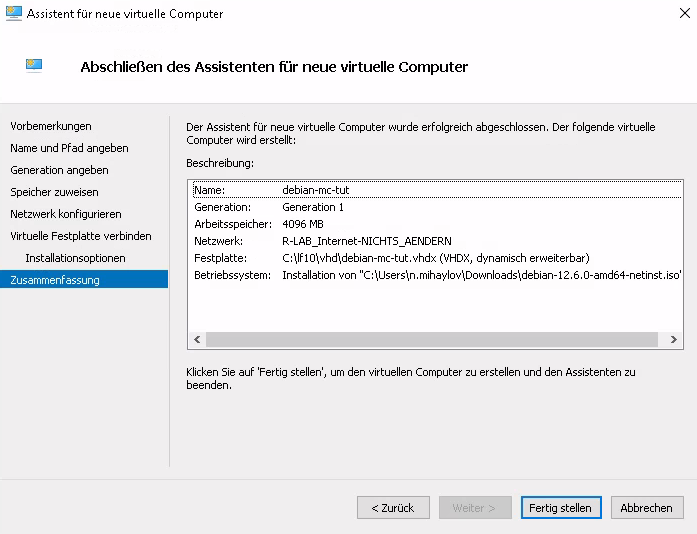
\includegraphics[width=1\textwidth]{vm-config}
\end{figure}
\FloatBarrier

\section{Herunterladen des neuesten Debian 12 Abbilds}

Die neueste Version des Debian 12 Abbilds kann von der offiziellen Website heruntergeladen werden \href{https://www.debian.org/download}{(hier klicken, um zur Download-Seite zu gelangen)}. Beachten Sie, dass wir für dieses Tutorial die netinst-Version verwenden, die eine Internetverbindung erfordert, um zusätzliche Pakete herunterzuladen, aber Sie können auch ein reguläres Komplettabbild für die Offline-Installation verwenden.

\section{Installationsprozess}

Die GUI-basierte Installation sollte relativ einfach sein - Sie können die Standardeinstellungen verwenden und den Hostnamen nach Belieben ändern (hier verwenden wir einfach "debian-mc"). Die Standardeinstellungen von Debian übernehmen die Festplattenpartitionierung auf unserer neuen VHDX. Stellen Sie sicher, dass Sie Ihre entsprechende Zeitzone, Sprache und Spiegelregion auswählen!

Einige Dinge, die für den Installationsprozess zu beachten sind: *nicht* eine Desktop-Umgebung installieren; wir benötigen nur eine SSH-Verbindung, um mit unserem Server zu interagieren, da wir die Belastung durch eine grafische Umgebung vermeiden wollen, daher sollten Sie nur "SSH-Server" und "Standard-Systemwerkzeuge" auswählen (siehe Abbildung 2 für ein visuelles Beispiel).

\begin{figure}[h]
    \caption{Unsere Debian 12 Softwareauswahl}
    \centering
    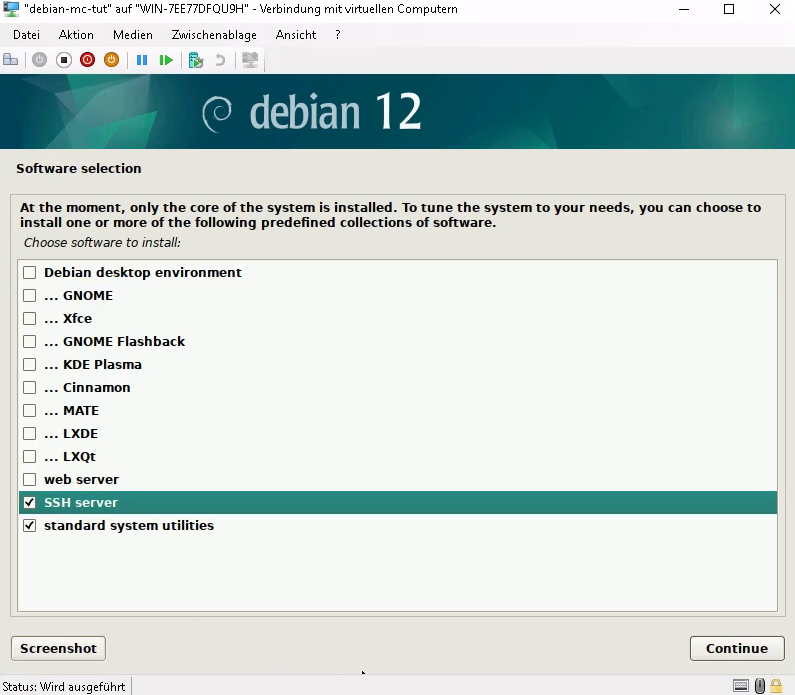
\includegraphics[width=1\textwidth]{debian-software-selection}
\end{figure}
\FloatBarrier

Der Grund, warum wir von Anfang an SSH haben möchten, ist, dass das Kopieren und Einfügen von Text viel einfacher wird, und Sie werden dies wahrscheinlich später während des Tutorials benötigen. Ein Benutzerkonto mit sudo-Rechten wird eine Voraussetzung für den SSH-Zugang sein, und nachdem Sie während der Installation ein Benutzerkonto erstellt haben, müssen Sie diese nur noch nach der Installation zur sudo-Gruppe hinzufügen.

Stellen Sie sicher, dass Sie den GRUB-Bootloader auf Ihrer primären Festplatte (/dev/sda) installieren, sonst können Sie nach der Installation nicht in Ihr System booten.

Jetzt sollten Sie eine funktionierende Debian 12 Installation mit einer TTY-Anmeldeaufforderung haben.

\begin{figure}[h!]
    \caption{Die Debian 12 TTY-Aufforderung}
    \centering
    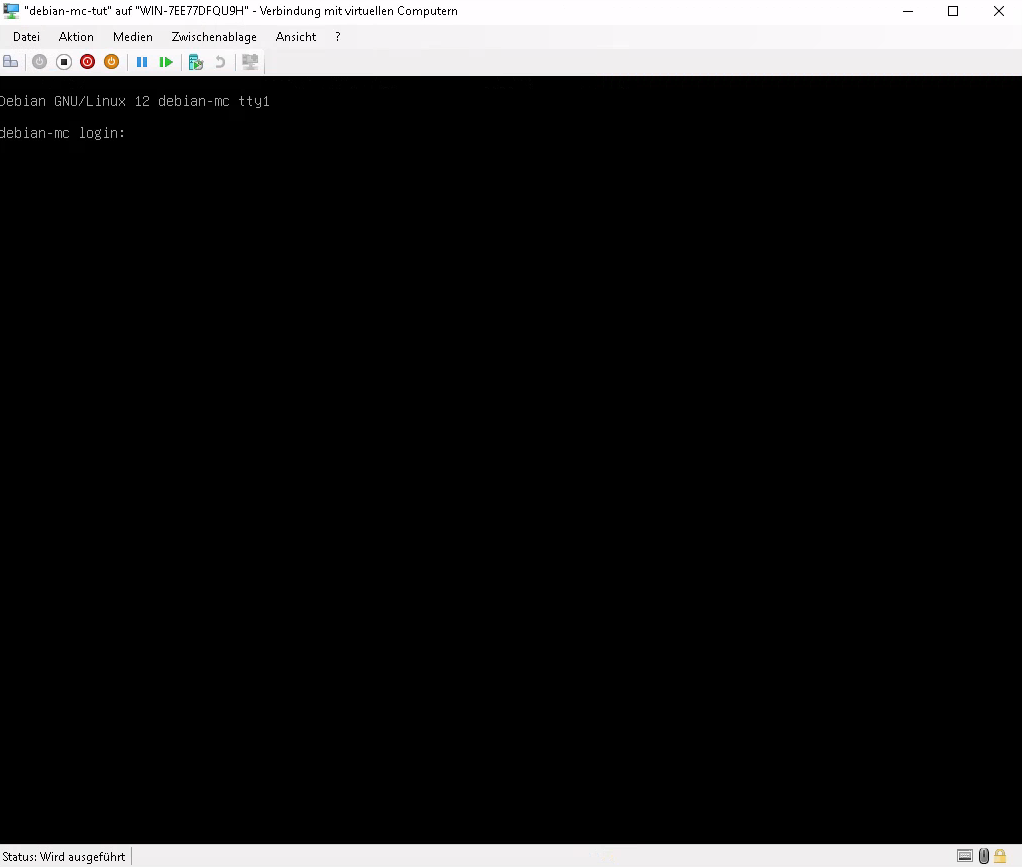
\includegraphics[width=1\textwidth]{tty}
\end{figure}
\FloatBarrier

\section{Erste Konfiguration nach der Installation}

Bevor wir mit etwas Minecraft-bezogenem beginnen, gibt es ein paar Dinge zu konfigurieren, wobei unser erstes und wichtigstes darin besteht, unserem neu erstellten Benutzer sudo-Rechte zu geben. Dazu melden wir uns als root an:

\begin{verbatim}
    debian-mc login: root
    Password: {your-root-password-here}
\end{verbatim}

Jetzt sollten Sie als root angemeldet sein und die Eingabeaufforderung sehen.

Das erste, was zu tun ist, ist das sudo-Paket zu installieren, falls es noch nicht installiert ist. Dazu geben wir Folgendes ein:

\begin{verbatim}
    apt install sudo
\end{verbatim}

Der apt-Befehl wird verwendet, um Pakete auf dem Debian-System zu verwalten. Mit dem Flag "install" können wir einen Paketnamen angeben, der installiert werden soll, in diesem Fall das sudo-Paket. Wenn sudo auf Ihrem System noch nicht verfügbar war, wird Ihr Paketmanager Sie fragen, ob Sie das Paket installieren möchten. Bestätigen Sie dies mit Enter. Sie können anschließend sudo eingeben, um zu bestätigen, dass das Paket installiert wurde, wobei die Hilfe für den Befehl ausgegeben wird.

Jetzt, da dies erledigt ist, können wir mit unserer grundlegenden Konfiguration fortfahren. Wir können alle Benutzer auf dem System mit dem folgenden Befehl auflisten:

\begin{verbatim}
    cat /etc/passwd
\end{verbatim}

Ihr neu erstellter Benutzer aus dem grafischen Installer wird höchstwahrscheinlich ganz unten stehen. Hier können Sie die lokalen Benutzerkonten pro Zeile und ihre zugehörige Benutzer-ID (UID), Gruppen-ID (GID), das Home-Verzeichnis, die Standard-Shell und mehr sehen.

\begin{figure}[h!]
    \caption{Ausgabe der /etc/passwd Datei}
    \centering
    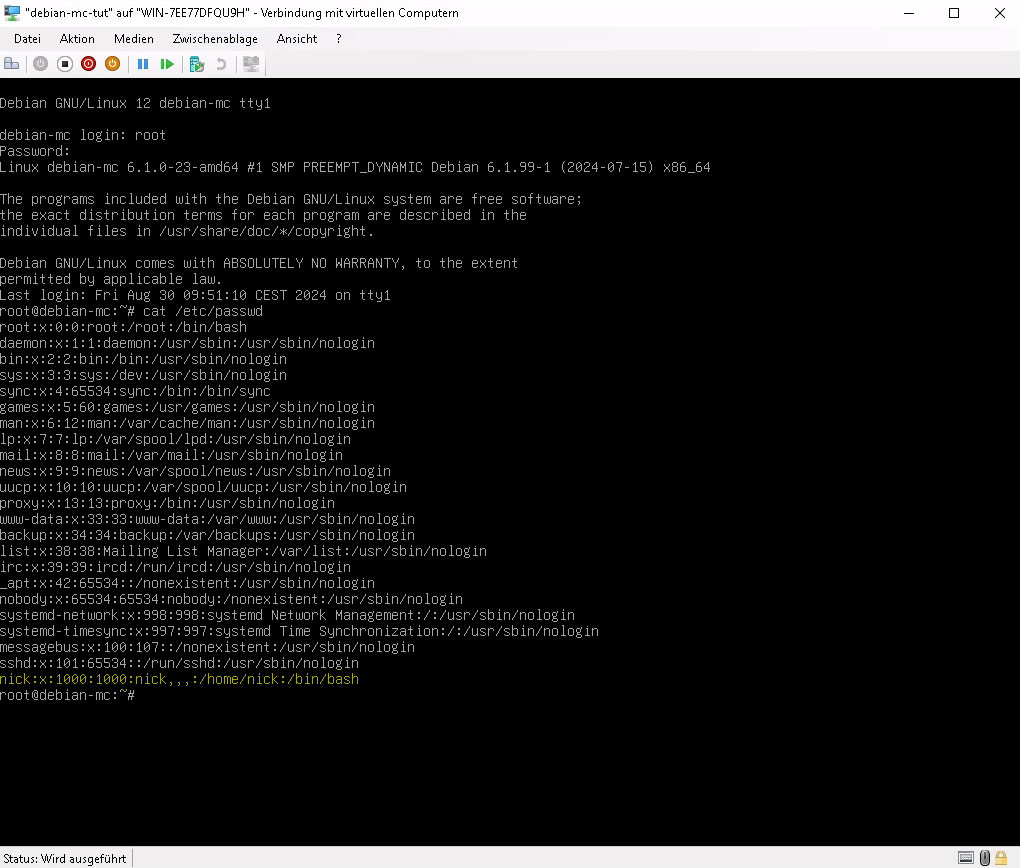
\includegraphics[width=1\textwidth]{passwd}
\end{figure}
\FloatBarrier

Jetzt werden wir unseren Benutzer zur sudo-Gruppe hinzufügen. Die sudo-Gruppe ist eine spezielle Gruppe, die über das sudo-Kommando administrative Rechte hat. Dazu geben wir den folgenden Befehl ein:

\begin{verbatim}
    usermod -aG sudo {your-username-here}
\end{verbatim}

Der Befehl usermod ermöglicht es uns, die Benutzerkonten zu ändern, die wir zuvor in der Datei /etc/passwd gesehen haben. Die Option -a steht für "append", also hinzufügen eines Benutzers zu einer Gruppe. Die Option -G dient zur Angabe einer Gruppe nach ihrem Namen (in diesem Fall sudo). In vielen GNU/Linux-Tools können Sie Optionen zusammenfassen, wie "-aG" statt "-a -G". Wenn Sie den Befehl eingegeben haben und keine Ausgabe erhalten haben, sollte alles in Ordnung sein.

Sie können jetzt mit dem Befehl su (Benutzer wechseln) zu Ihrem Benutzer zurückwechseln, um Ihre neu erhaltenen sudo-Rechte zu testen:

\begin{verbatim}
    su {your-username-here}
\end{verbatim}

Versuchen Sie nun, Ihr System mit sudo zu aktualisieren:

\begin{verbatim}
    sudo apt update && sudo apt upgrade
\end{verbatim}

Wenn alles gut gelaufen ist, sollten Sie Ihr System mit dem apt-Repository synchronisieren und alle verfügbaren Updates auf Ihrem Computer installieren können!

\begin{figure}[h!]
    \caption{Testen der neu vergebenen sudo-Rechte durch Aktualisierung unseres Systems}
    \centering
    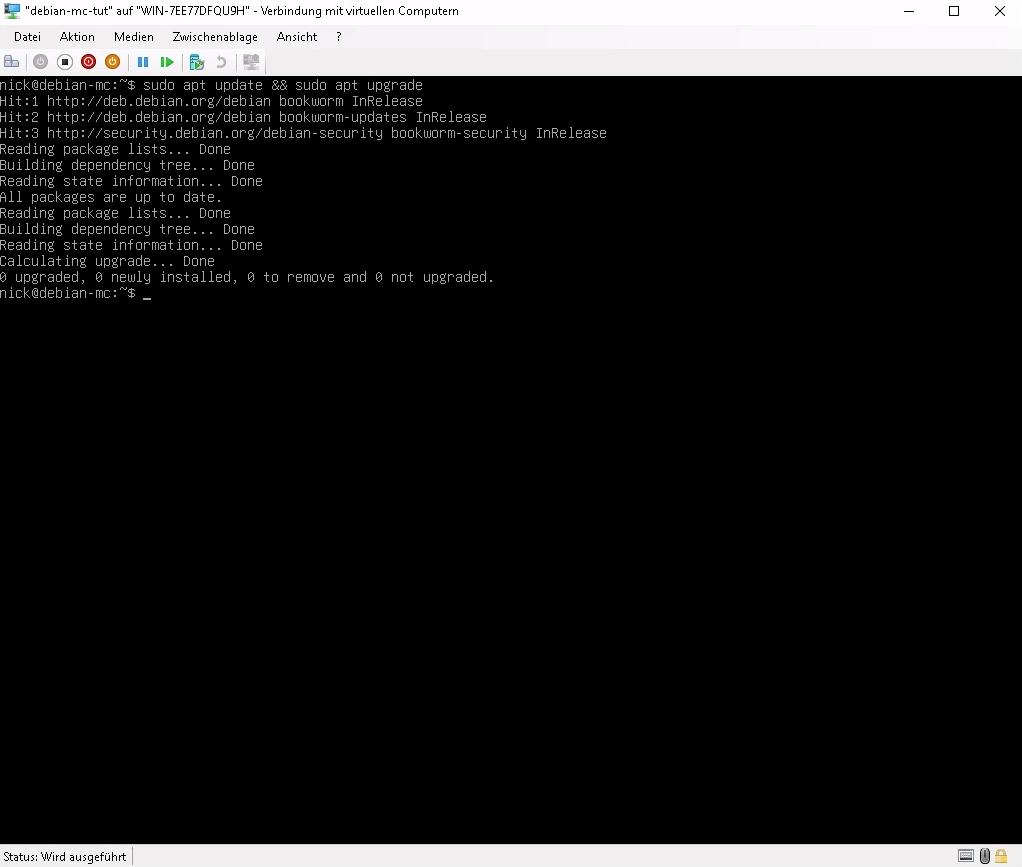
\includegraphics[width=1\textwidth]{update}
\end{figure}
\FloatBarrier

\section{Herstellen einer SSH-Verbindung}

Wenn Sie den Installationsabschnitt dieses Tutorials befolgt haben, haben Sie höchstwahrscheinlich OpenSSH installiert, das für diesen Abschnitt erforderlich ist. Um dies zu überprüfen, können Sie den folgenden Befehl ausführen:

\begin{verbatim}
    ssh
\end{verbatim}

Sie erhalten nun die Hilfe-Ausgabe des Befehls, wenn das OpenSSH-Paket auf Ihrem System installiert ist. Wenn nicht, installieren Sie es mit dem folgenden Befehl:

\begin{verbatim}
    sudo apt install openssh-server
\end{verbatim}

Wenn dies abgeschlossen ist, können wir zu unserem Host-System zurückkehren und ein Befehlszeilenfenster öffnen (z.B. PowerShell). Um eine Verbindung herzustellen, müssen wir eine bestimmte Syntax befolgen:

\begin{verbatim}
    ssh {username}@{ipv4-address}
\end{verbatim}

Wir verbinden uns als Benutzer auf unserem SSH-Server unter der angegebenen IPv4-Adresse des Servers. Wenn Sie Ihre IPv4-Adresse nicht kennen, können Sie den folgenden Befehl ausführen, um die IPv4-Adresse Ihres Ethernet-Adapters/NIC zu erhalten:

\begin{verbatim}
    ip addr | grep "eth0"
\end{verbatim}

Der Befehl "ip addr" gibt Informationen zu den Netzwerkschnittstellen des Systems aus. Da wir mit einer VM arbeiten, ist es sehr wahrscheinlich, dass wir einen virtuellen Ethernet-Adapter verwenden, daher verwenden wir standardmäßig "eth0", um die Informationen zu erhalten. Wenn Sie normalerweise "ip addr" ausführen, werden alle Schnittstellen angezeigt, was bei unserer frischen Installation kein Problem darstellen sollte. Wenn Sie jedoch mit Befehlen arbeiten, die viele Informationen ausgeben, von denen wir nur einen kleinen Teil benötigen, können wir gleichzeitig den Befehl "grep" verwenden. Dieses Hilfsprogramm durchsucht die Ausgabe Ihres vorherigen Befehls (in unserem Fall "ip addr") und gibt nur die Zeile aus, die als Argument für grep angegeben ist (in diesem Fall "eth0").

Die Pipe zwischen diesen beiden Befehlen ist der wichtigste Teil; dies sollte Ihre Einführung in das Konzept der Ein-/Ausgabeumleitung in Linux sein, wobei die Pipe die Ausgabe unseres linken Befehls nimmt und sie als Eingabe an den rechten Befehl weitergibt. Grob gesagt sieht der Ablauf dieses gesamten Befehls nun folgendermaßen aus: \texttt{"ip addr" -> | -> "grep 'eth0'"}.

Ihre Ausgabe sollte etwa so aussehen:

\begin{figure}[h!]
	\caption{Die Ausgabe des \texttt{ip addr | grep "eth0"}-Befehls}
	\centering
	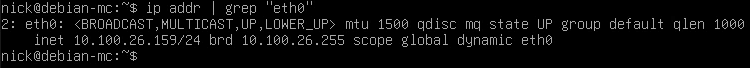
\includegraphics[width=1\textwidth]{ip-addr}
\end{figure}
\FloatBarrier

Mit unserer IP-Adresse in der Hand können wir nun unseren bevorzugten Terminal-Emulator verwenden und die Syntax von früher verwenden, um uns von unserem Host aus mit unserer Maschine zu verbinden:

\begin{figure}[h!]
	\caption{Herstellen einer SSH-Verbindung zur VM}
	\centering
	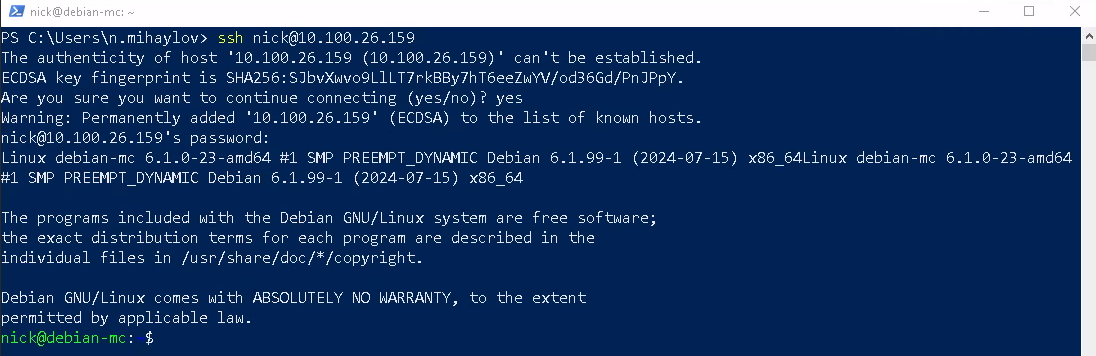
\includegraphics[width=1\textwidth]{ssh}
\end{figure}
\FloatBarrier

Erfolg! Sie sollten nun eine SSH-Verbindung zu Ihrer Debian 12-VM haben. Natürlich ist es wichtig zu beachten, dass sich die Maschinen im selben Netzwerk befinden sollten, aber Sie können so weit gehen, dass Sie anstelle von RemoteLabs einen Terminal-Emulator auf Ihrem von GFN ausgestellten Laptop verwenden, um sich über SSH mit der VM zu verbinden. Damit können Sie jetzt lange Befehle einfach in Ihre VM kopieren und einfügen, ohne sie manuell eingeben zu müssen.

\section{Vorbereitung der Minecraft Forge Server-Installation}

Um unsere Instanz von Forge für den Minecraft-Server zu hosten, benötigen wir eine Installation des Java Development Kit auf unserem System.

Hier entsteht ein Problem: Die neueste Version von Forge erfordert Version 21 des JDK, aber diese Version von OpenJDK befindet sich zum Zeitpunkt des Schreibens dieses Dokuments noch im Test-Repository, und das Oracle JDK ist unter deren eigener Lizenz lizenziert und ebenfalls nicht in den Repositories verfügbar. An dieser Stelle muss ich klarstellen, dass dies nicht in einer Produktionsumgebung verwendet werden sollte, allein wegen der unübersichtlichen Java-Situation auf Debian.

Das alles vorausgeschickt, wird dieses Dokument mit der Oracle JDK 21 .deb-Datei fortfahren, die \href{https://www.oracle.com/java/technologies/downloads/}{(hier)} gefunden werden kann. Kopieren Sie den Link zur .deb-Datei von dieser Seite und halten Sie ihn in Ihrer Zwischenablage.

Zurück zur eingerichteten SSH-Verbindung zu unserem Debian 12 müssen wir einen Ordner erstellen, um unsere heruntergeladene Datei zu speichern. Dazu navigieren wir zuerst in das Home-Verzeichnis unseres Benutzers, indem wir einfach "cd" eingeben (Sie können mit dem Befehl "pwd" überprüfen, in welchem Verzeichnis Sie sich gerade befinden), und dann den Befehl "mkdir" (Verzeichnis erstellen) innerhalb unseres Home-Verzeichnisses verwenden, um ein neues wie folgt zu erstellen:

\begin{verbatim}
	mkdir Downloads
\end{verbatim}

Wenn wir nun ein "ls" (Liste) ausführen, sollten wir sehen, dass das neue Verzeichnis mit dem Namen "Downloads" erstellt wurde.

\begin{figure}[h!]
	\caption{Erstellen eines Verzeichnisses im Home-Verzeichnis des Benutzers}
	\centering
	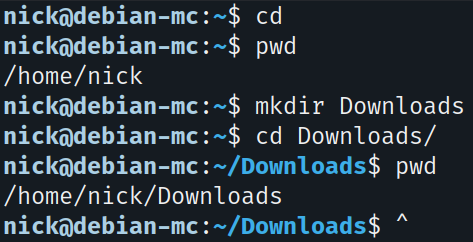
\includegraphics[width=1\textwidth]{downloads}
\end{figure}
\FloatBarrier

An diesem Punkt können wir die JDK .deb-Datei, die wir derzeit in unserer Zwischenablage haben, mit dem Tool "wget" herunterladen. Der Befehl sollte ziemlich einfach sein, jetzt wo wir dank SSH eine funktionierende Zwischenablage zur Hand haben:

\begin{verbatim}
	wget https://download.oracle.com/java/22/latest/jdk-22_linux-x64_bin.deb
\end{verbatim}

Der obige Link ist für das Oracle JDK 22. Je nachdem, wann Sie dieses Dokument lesen, könnte das OpenJDK 21-Paket bereits im stabilen Repository von Debian verfügbar sein. Im Rest des Tutorials werden wir mit der heruntergeladenen .deb-Datei von Oracle fortfahren.

Wenn Sie ein "ls" in Ihrem Downloads-Verzeichnis ausführen, sollten Sie die Datei sehen, die Sie gerade mit "wget" heruntergeladen haben:

\begin{figure}[h!]
	\caption{Die heruntergeladene JDK .deb-Datei}
	\centering
	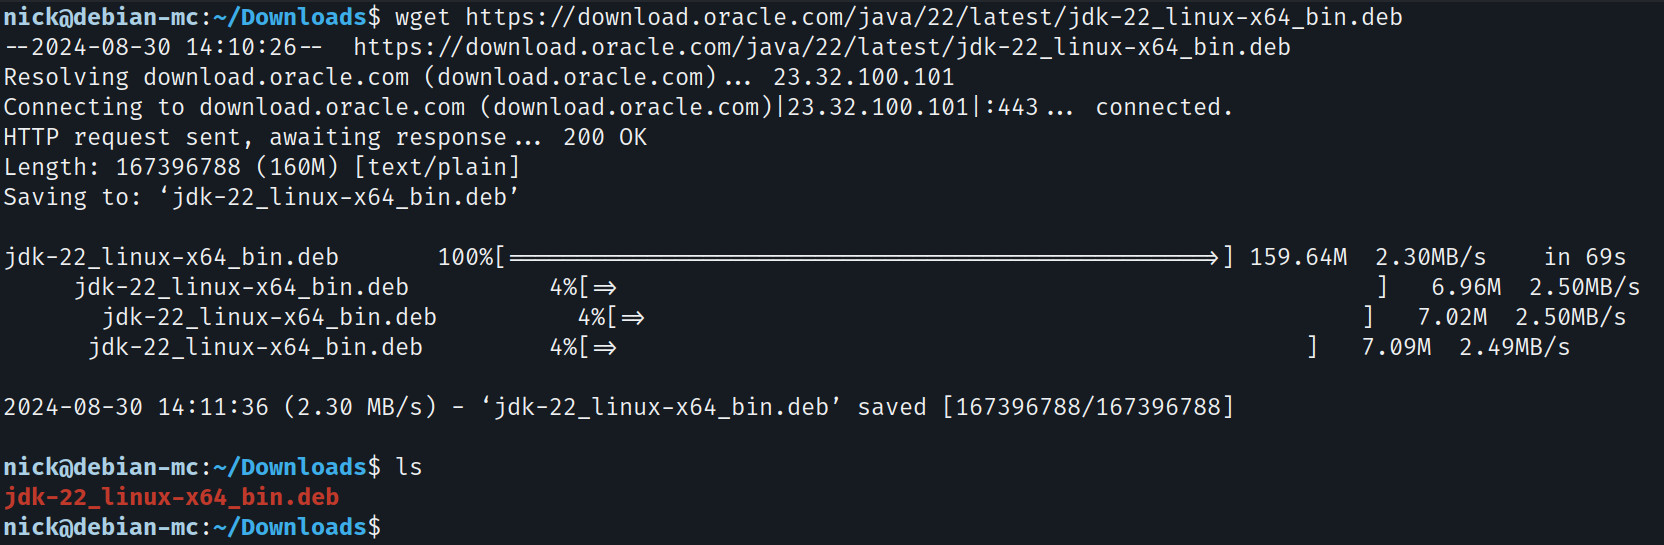
\includegraphics[width=1\textwidth]{wget}
\end{figure}
\FloatBarrier

Dateien mit der Endung .deb sind vergleichbar mit einer Windows .exe-Installationsdatei - sie enthalten die benötigten Binärdateien und Daten für eine Anwendung sowie alle notwendigen Meta-Informationen für das System. Tatsächlich können Sie diese Datei mit einem Archivbetrachter öffnen und sehen, dass sie aus zwei Tarball-Archiven besteht, jeweils für die Anwendung selbst und ihre Metadaten.

Um eine .deb-Datei als Systempaket zu installieren, benötigen wir den Befehl "dpkg". "apt" verwendet tatsächlich "dpkg" im Hintergrund, um die Installation von Paketen durchzuführen, aber jetzt überspringen wir "apt" und gehen direkt zu "dpkg", um eine Datei zu installieren. Wir verwenden den folgenden Befehl:

\begin{verbatim}
	sudo dpkg -i jdk-22_linux-x64_bin.deb
\end{verbatim}

Denken Sie daran, dass Sie die Tab-Vervollständigung verwenden können! Beginnen Sie mit den ersten Buchstaben des Dateinamens und verwenden Sie die Tabulatortaste, um den Rest automatisch auszufüllen. Sie werden nach Ihrem sudo-Passwort gefragt und die Installation sollte beginnen.

Wenn die Installation abgeschlossen ist, wird es alle möglichen Ausgaben auf Ihrem Terminal geben. Wenn es ähnlich wie in der folgenden Abbildung aussieht, sollten Sie gut sein.

\begin{figure}[h!]
	\caption{Ausgabe der JDK .deb-Installation}
	\centering
	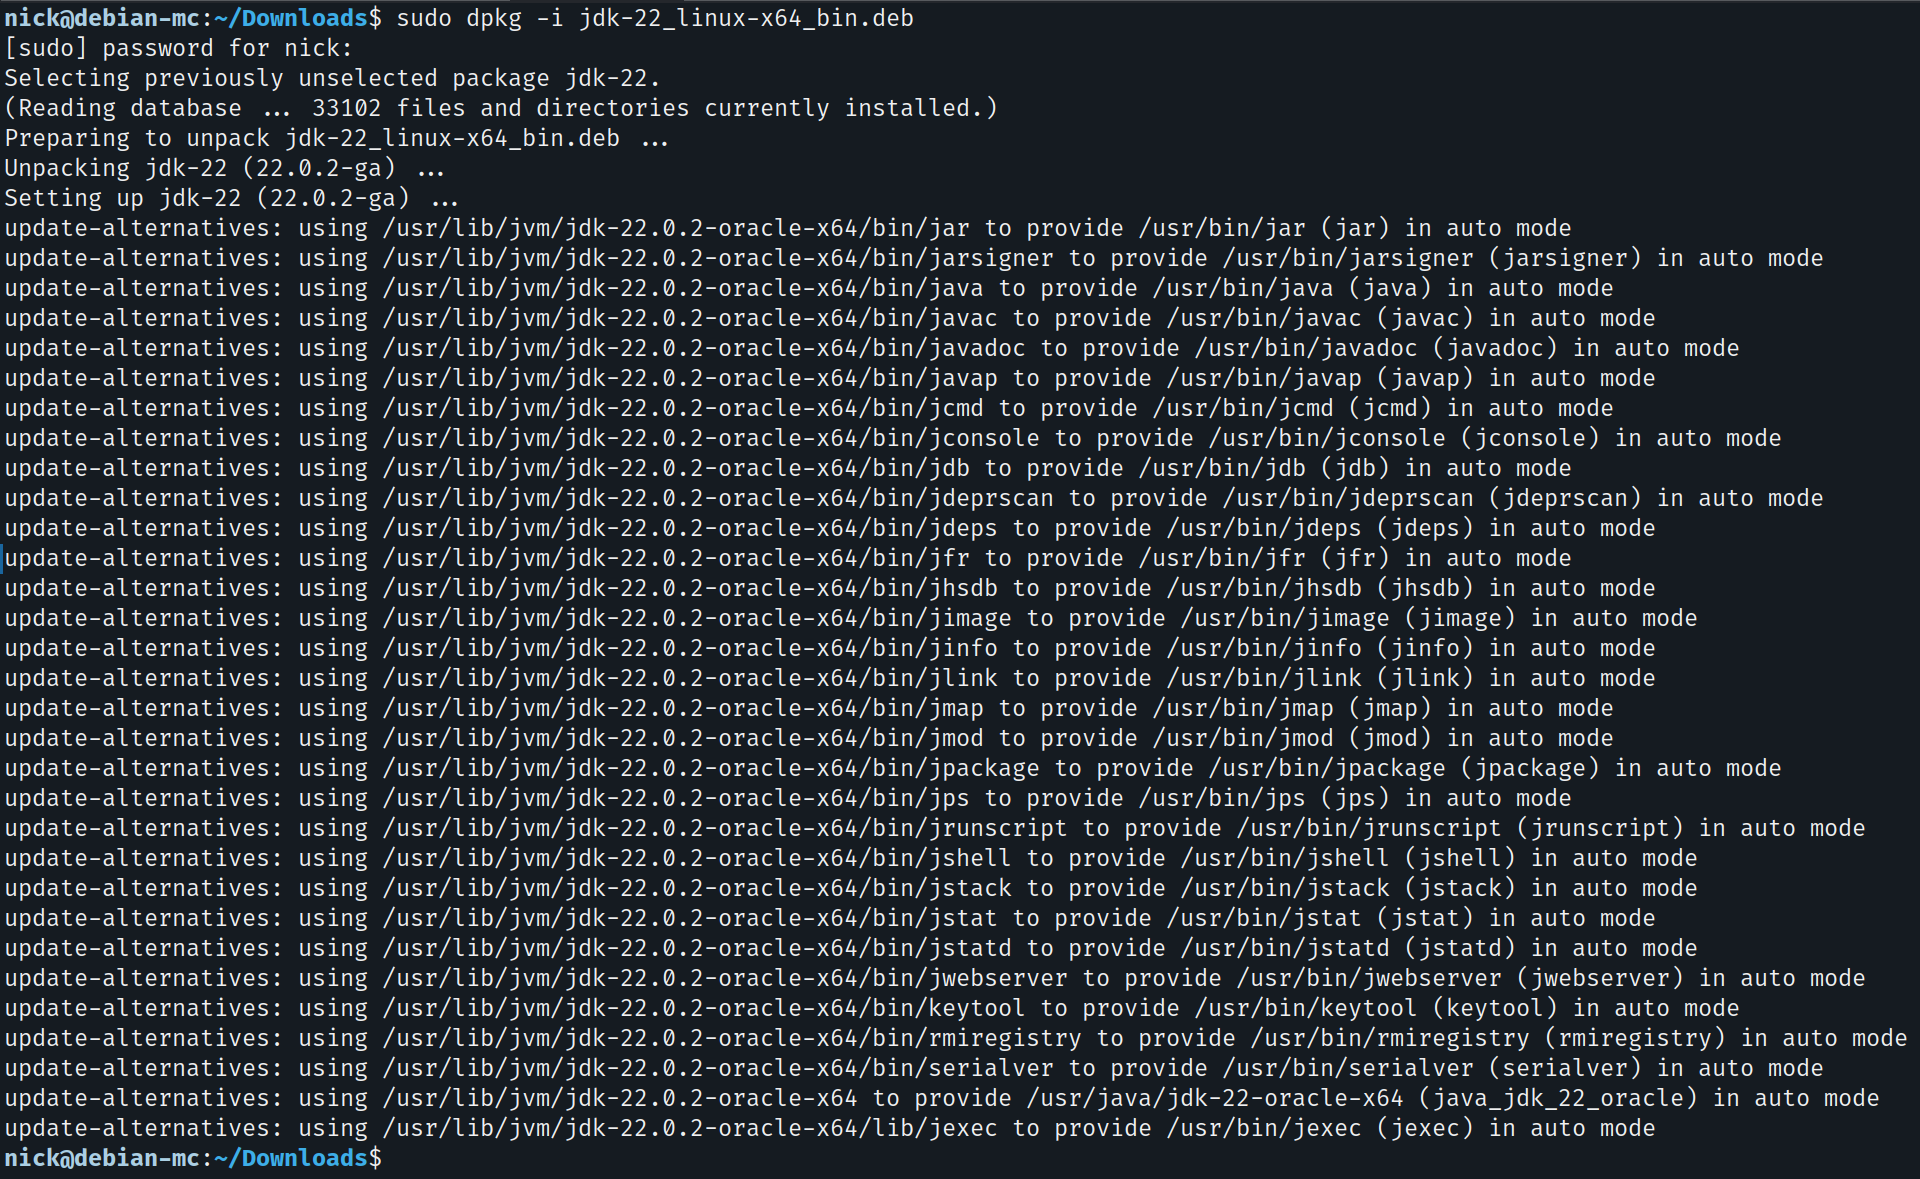
\includegraphics[width=1\textwidth]{jdk-output}
\end{figure}
\FloatBarrier

Sie können die Installation überprüfen, indem Sie \texttt{java --version} ausführen, was hoffentlich die Version des Pakets anzeigt, das Sie gerade installiert haben (in diesem Fall 22.0.2). Sie haben nun erfolgreich das benötigte Java JDK für die Ausführung von Forge installiert!

\section{Installation von Minecraft Forge}

Wir sollten zuerst ein dediziertes Verzeichnis für unsere Minecraft-Installation erstellen und in dieses wechseln:

\begin{verbatim}
	sudo mkdir /opt/minecraft
	cd /opt/minecraft
\end{verbatim}

Jetzt können wir mit "wget" die neueste empfohlene Version von Forge herunterladen, die zum Zeitpunkt des Schreibens dieses Dokuments verfügbar ist. Diese können Sie von \href{https://maven.minecraftforge.net/net/minecraftforge/forge/1.20.6-50.1.0/forge-1.20.6-50.1.0-installer.jar}{(hier)} beziehen. Wenn Sie "wget" mit diesem Link als Argument ausführen, wird die Datei in unserem Verzeichnis \texttt{/opt/minecraft} heruntergeladen:

\begin{verbatim}
	sudo wget https://maven.minecraftforge.net/.../...installer.jar
\end{verbatim}

Überprüfen Sie mit einem "ls", ob die Datei im aktuellen Verzeichnis heruntergeladen wurde. Wir können nun mit der Installation der Server-Version von Minecraft Forge mit der .jar-Datei unter Verwendung von Java fortfahren:

\begin{verbatim}
	sudo java -jar forge-1.20.6-50.1.0-installer.jar --installServer
\end{verbatim}

Dieser Vorgang kann eine Weile dauern. Sie wissen, dass er erfolgreich abgeschlossen wurde, wenn die Meldung "The server installed successfully" am Ende erscheint.

Der nächste Schritt besteht darin, eine "eula.txt"-Datei zu erstellen, die vom Minecraft-Server benötigt wird. Wir können entweder die Datei mit "touch" erstellen, um sie ohne Inhalt zu erstellen, oder sie mit einem Texteditor wie "nano" erstellen, da wir den Inhalt ohnehin in die Datei schreiben müssen.

Durch "Touching" einer Datei wird eine leere Datei mit dem Namen erstellt, den Sie dem Touch-Befehl angegeben haben, wie folgt:

\begin{verbatim}
	sudo touch eula.txt
\end{verbatim}

Wenn Sie nun das Verzeichnis mit "ls" auflisten, sollten Sie die Datei sehen. Wenn Sie ihren Inhalt mit "cat" ausgeben, werden Sie nichts sehen, da sie leer ist. Zum Bearbeiten verwenden wir den Texteditor "nano":

\begin{verbatim}
	sudo nano eula.txt
\end{verbatim}

Jetzt befinden Sie sich in der Benutzeroberfläche des nano-Texteditors:

\begin{figure}[h!]
	\caption{Der nano-Texteditor}
	\centering
	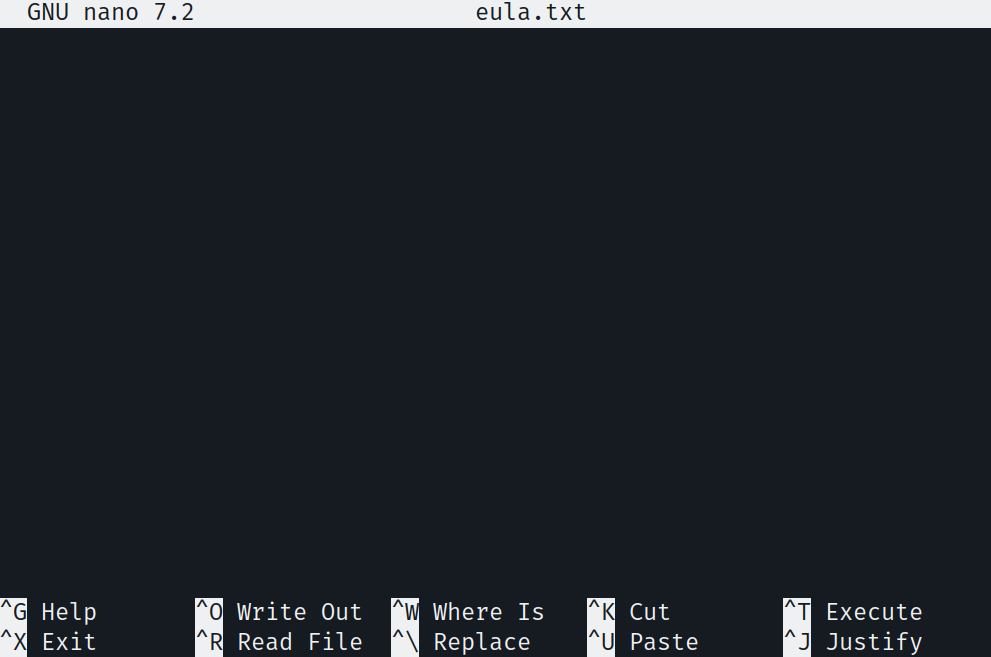
\includegraphics[width=1\textwidth]{nano}
\end{figure}
\FloatBarrier

nano ist ein relativ einfacher Texteditor - Sie können direkt loslegen und Text in den Editor-Puffer schreiben und ihn mit Strg+O speichern, um ihn "auszuschreiben", und mit Enter bestätigen. Hier müssen wir nur die folgende Zeile hinzufügen:

\begin{verbatim}
	eula=true
\end{verbatim}

Schreiben Sie den Puffer mit Strg+O in die Datei und drücken Sie Enter, um unter dem Standarddateinamen zu speichern. Wenn beim Speichern ein Fehler auftritt, haben Sie wahrscheinlich vergessen, nano als Superuser mit dem sudo-Befehl zu starten.

Wenn Sie immer noch Lust auf Ausgabeumleitung haben, können wir das Verwenden von "nano" überspringen und unsere Bash-Shell diese Zeile mit diesem Befehl in unsere Datei schreiben lassen:

\begin{verbatim}
	echo "eula=true" | sudo tee -a eula.txt
\end{verbatim}

Der Befehl "echo" gibt alles, was danach kommt, in die Shell aus, aber die Pipe nimmt diese Ausgabe und übergibt sie an "tee" mit sudo-Rechten, um sie mit dem -a-Flag an die eula.txt-Datei anzuhängen. Der Befehl "tee" ist ein Dienstprogramm, das die Ausgabe eines Befehls liest, sie auf dem Bildschirm anzeigt und sie auch in eine Ausgabedatei schreibt (in diesem Fall die "eula.txt"). Während es bequemer ist, diese Zeile mit einem Texteditor wie nano zu unserer Datei hinzuzufügen, ist das Konzept der Umleitung wichtig, wenn es darum geht, Skripte zu erstellen, die Ihnen auf Ihrer Linux-Reise nützlich sein könnten.

Wir können den Inhalt der Datei mit "cat" überprüfen, das das, was wir gerade in die Datei geschrieben haben, ausgeben sollte.

Lassen Sie uns nun eine leere Datei "server.properties" mit "touch" erstellen:

\begin{verbatim}
	touch server.properties
\end{verbatim}

Lassen Sie uns auch eine vorhandene Datei in diesem Verzeichnis mit dem Namen \texttt{user\_jvm\_args.txt} ändern. Diese Datei sollte die Anweisungen enthalten, wie die Java Virtual Machine gestartet werden soll.

\begin{verbatim}
	sudo nano user_jvm_args.txt
\end{verbatim}

Alle Zeilen, die mit einem \# beginnen, werden ignoriert, da sie als Kommentare interpretiert werden; alles, was danach folgt und kein \# hat, wird als Eintrag in der Konfigurationsdatei gelesen. Wir müssen nur Folgendes hinzufügen:

\begin{verbatim}
	-Xms4G
	-Xmx4G
\end{verbatim}

Damit wird der JVM mindestens 4 GB und maximal 4 GB RAM zugewiesen. Beachten Sie, dass die ersten X's groß geschrieben sind.

Alles, was noch zu tun ist, ist die "run.sh"-Shell-Skriptdatei zu bearbeiten, um die allerletzte Zeile zu ändern, indem wir \texttt{cd /opt/minecraft \&\&} am Anfang der Zeile hinzufügen und ein \texttt{nogui} anhängen.

Ihre Datei sollte nun so aussehen:

\begin{figure}[h!]
	\caption{Der Inhalt der bearbeiteten run.sh-Datei}
	\centering
	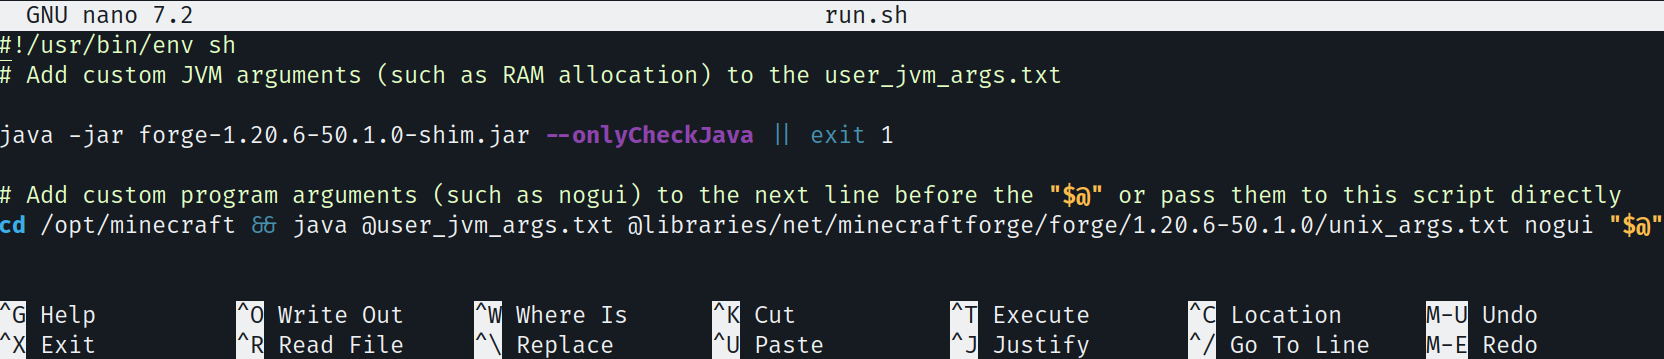
\includegraphics[width=1\textwidth]{run-sh}
\end{figure}
\FloatBarrier

Wenn hoffentlich alles abgeschlossen ist, können wir endlich das Shell-Skript ausführen, um unseren Minecraft-Server zu starten:

\begin{verbatim}
	sudo sh run.sh
\end{verbatim}

Dieser Vorgang dauert eine Weile, insbesondere während der Weltgenerierungsphase. Sie werden wissen, dass es fertig ist, wenn die Meldung "Done" und das >-Zeichen der Minecraft-Konsolen-Eingabeaufforderung erscheinen, sobald alles eingerichtet ist. Sie können nun versuchen, sich mit Ihrem neu erstellten Minecraft-Server zu verbinden, wobei Sie beachten sollten, dass Sie möglicherweise eine bestimmte Version des Clients benötigen (in diesem Fall habe ich die Client-Version 1.26.0 verwendet, die vom Prism Launcher verwaltet wird).

\begin{figure}[h!]
	\caption{Beitritt zum Server mit der IPv4-Adresse}
	\centering
	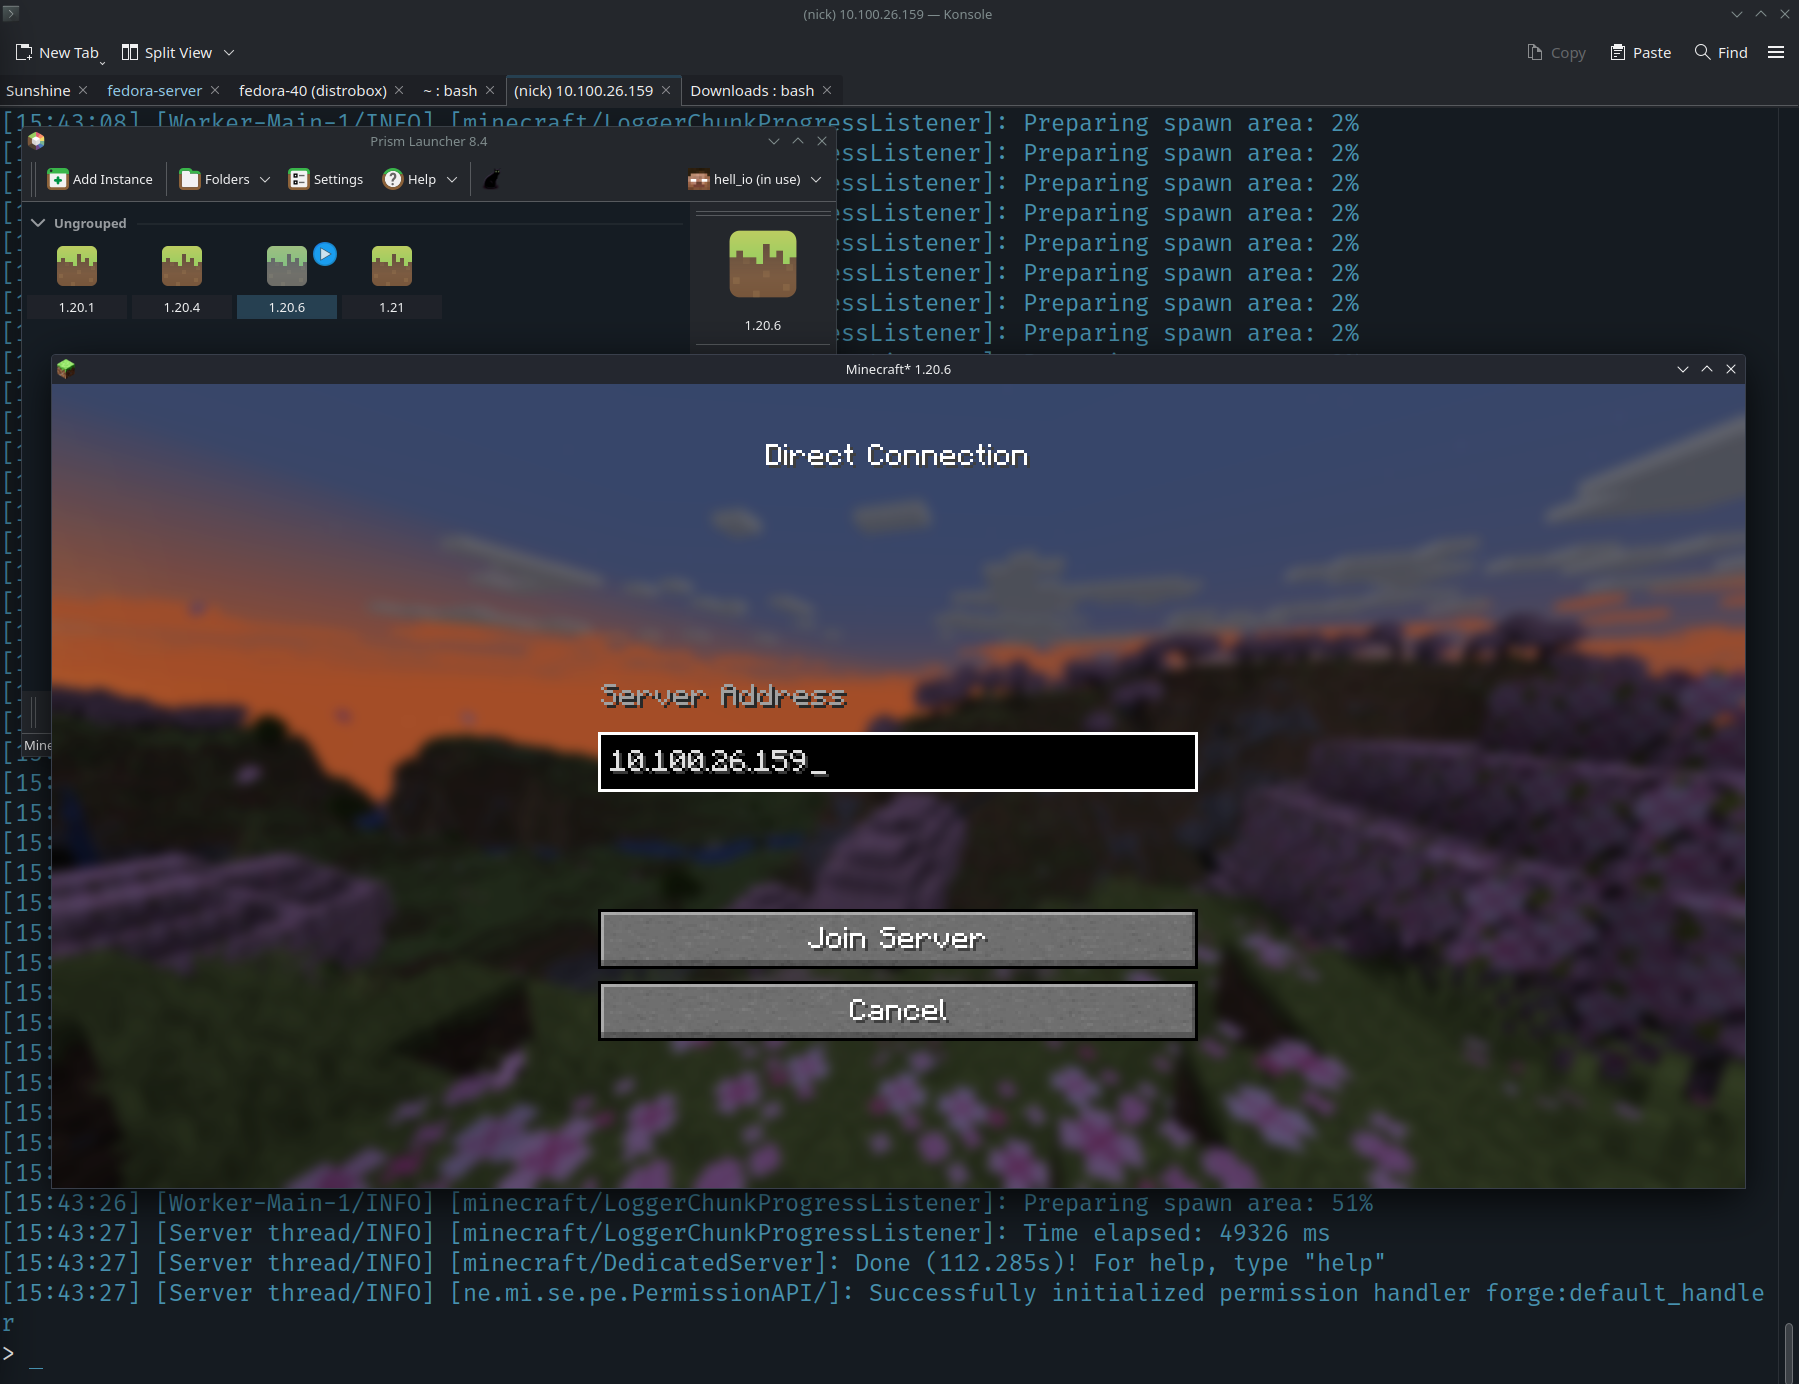
\includegraphics[width=0.8\textwidth]{mc-connect}
\end{figure}
\FloatBarrier

\begin{figure}[h!]
	\caption{Screenshot des Servers und des generierten Seeds im Spiel}
	\centering
	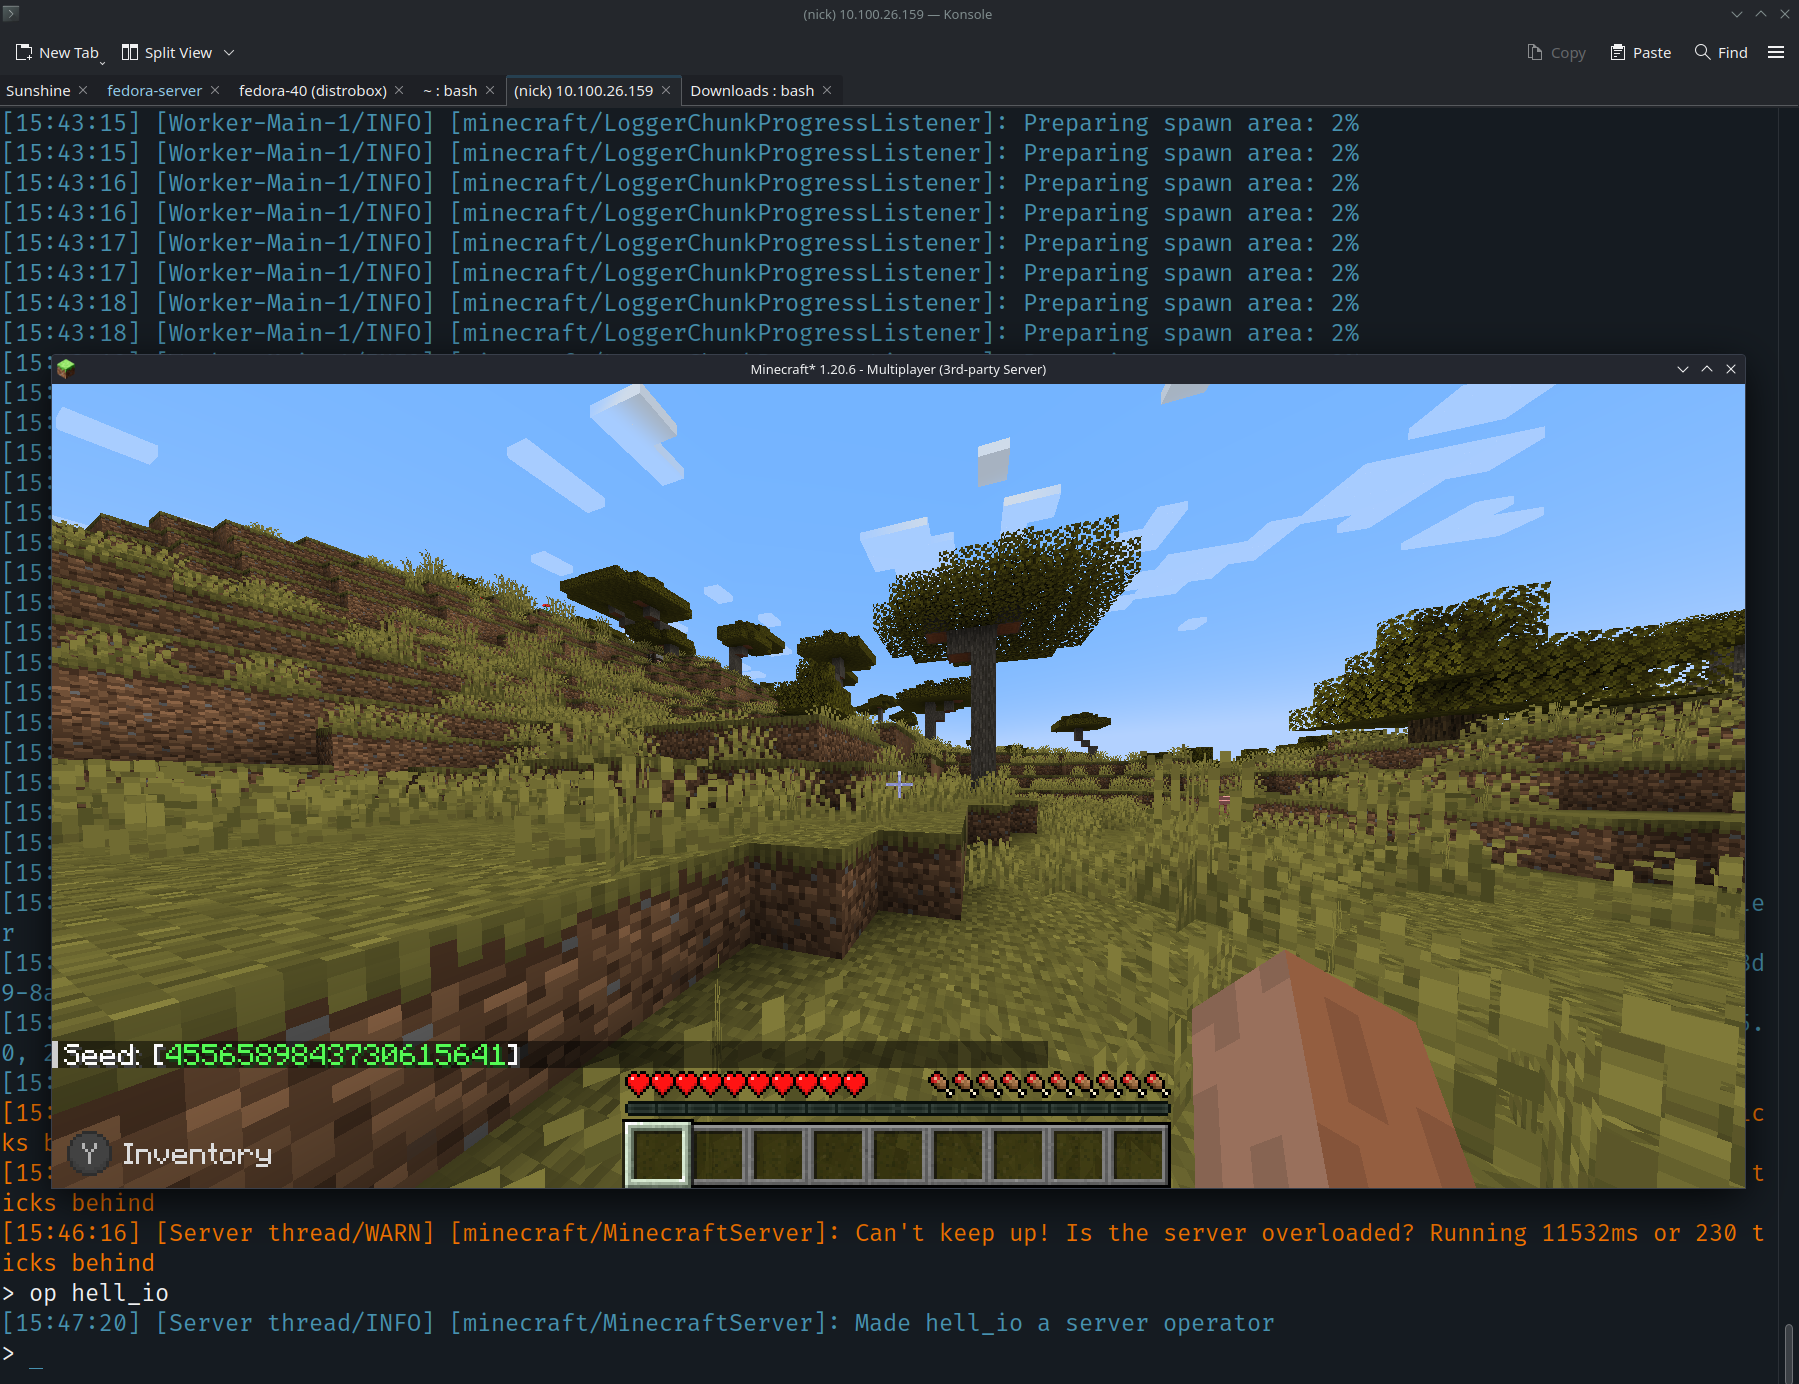
\includegraphics[width=0.8\textwidth]{mc-server}
\end{figure}
\FloatBarrier

Herzlichen Glückwunsch! Sie sollten nun einen funktionierenden Minecraft Forge-Server auf Ihrer Debian 12-VM haben!

\end{document}
